\chapter{OpenDQ hardware}
\label{sec:02-hardware}
As stated earlier, the OpenDQ project is designed to run on the OpenMote platform. The OpenMote platform is composed of three different boards: the OpenMote-CC2538, the OpenBase and OpenBattery. These boards are described in the following subsections. In addition to OpenDQ, the OpenMote-CC2538 and its companion boards can also run different operating systems and stacks for the IoT (Internet of Things). In particular, the OpenMote boards are fully compatible with Contiki ($http://www.contiki-os.org/$) and OpenWSN ($http://openwsn.berkeley.edu/$), and are partially supported by RioT ($http://www.riot-os.org/$).

%%
% OpenMote-CC2538
%%
\section{OpenMote-CC2538}
The OpenMote-CC2538 board, depicted in Figure~\ref{fig:openmote-cc2538}, is the core of the OpenMote platform. It has an XBee Pro form factor and embeds the Texas Insturments SoC (System On Chip) \cite{cc2538ds, cc2538ug} that embeds a 32-bit ARM Cortex-M3 micro-controller and an IEEE~802.15.4 radio transceiver operating at the 2.45~GHz band. The micro-controller runs up to 32 MHz and includes 32 kbytes of RAM and 512 kbytes of Flash memory, as well as different peripherals (GPIOs, UART, SPI, I2C, ADC, Timers, etc.). The OpenMote-CC2538 also contains four LEDs (green, yellow, orange and red), two buttons (reset and user) and a SMA antenna connector. The OpenMote-CC2538 is intended to be plugged to the OpenBase and the OpenBattery boards to complete its functionality; for example, the OpenMote-CC2538 can be connected to a computer for debugging purposes using an OpenBase. The schematic of the OpenMote-CC2538 board can be found online in \cite{openmote_schematic}.

% OpenMote-CC2538 board
\begin{figure}[!ht]
    \centering
	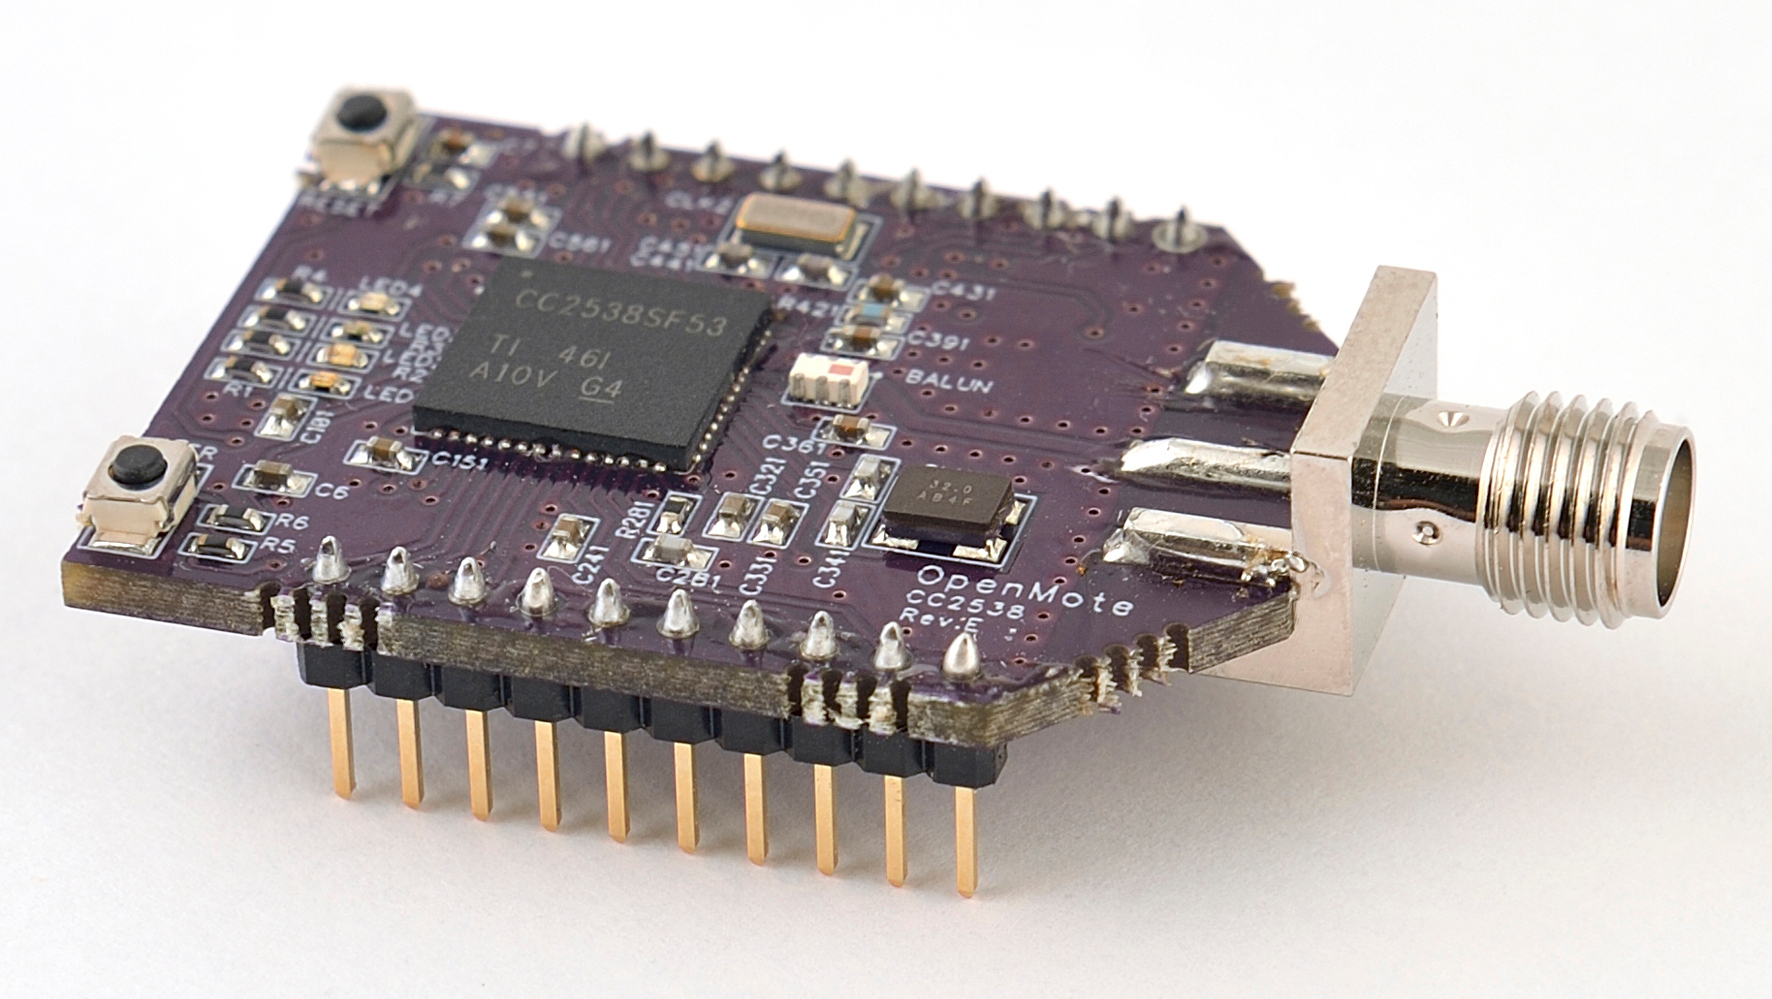
\includegraphics[width=0.45\linewidth]{01-openmote}
    \caption{OpenMote-CC2538 board.}
    \label{fig:openmote-cc2538}
\end{figure}

%%
% OpenBase
%%
\section{OpenBase}
The OpenBase board, depicted in Figure~\ref{fig:openbase}, serves as an interconnect board that provides connectivity and debugging capabilities for the OpenMote-CC2538 board. Regarding connectivity, the OpenBase provides a UART interface, a USB interface and a Ethernet interface. Power to the OpenBase can be provided via either USB port, i.e., USB\_FTDI and USB\_CC2538, and can be selected via the power switch. Regarding debugging, the OpenBase provides full access to the XBee pins, an ARM JTAG 10-pin connector and a current probe to measure the current consumption of the OpenMote-CC2538. The schematic of the OpenBase board can be found online in \cite{openbase_schematic}.

% OpenBase board
\begin{figure}[!ht]
    \centering
	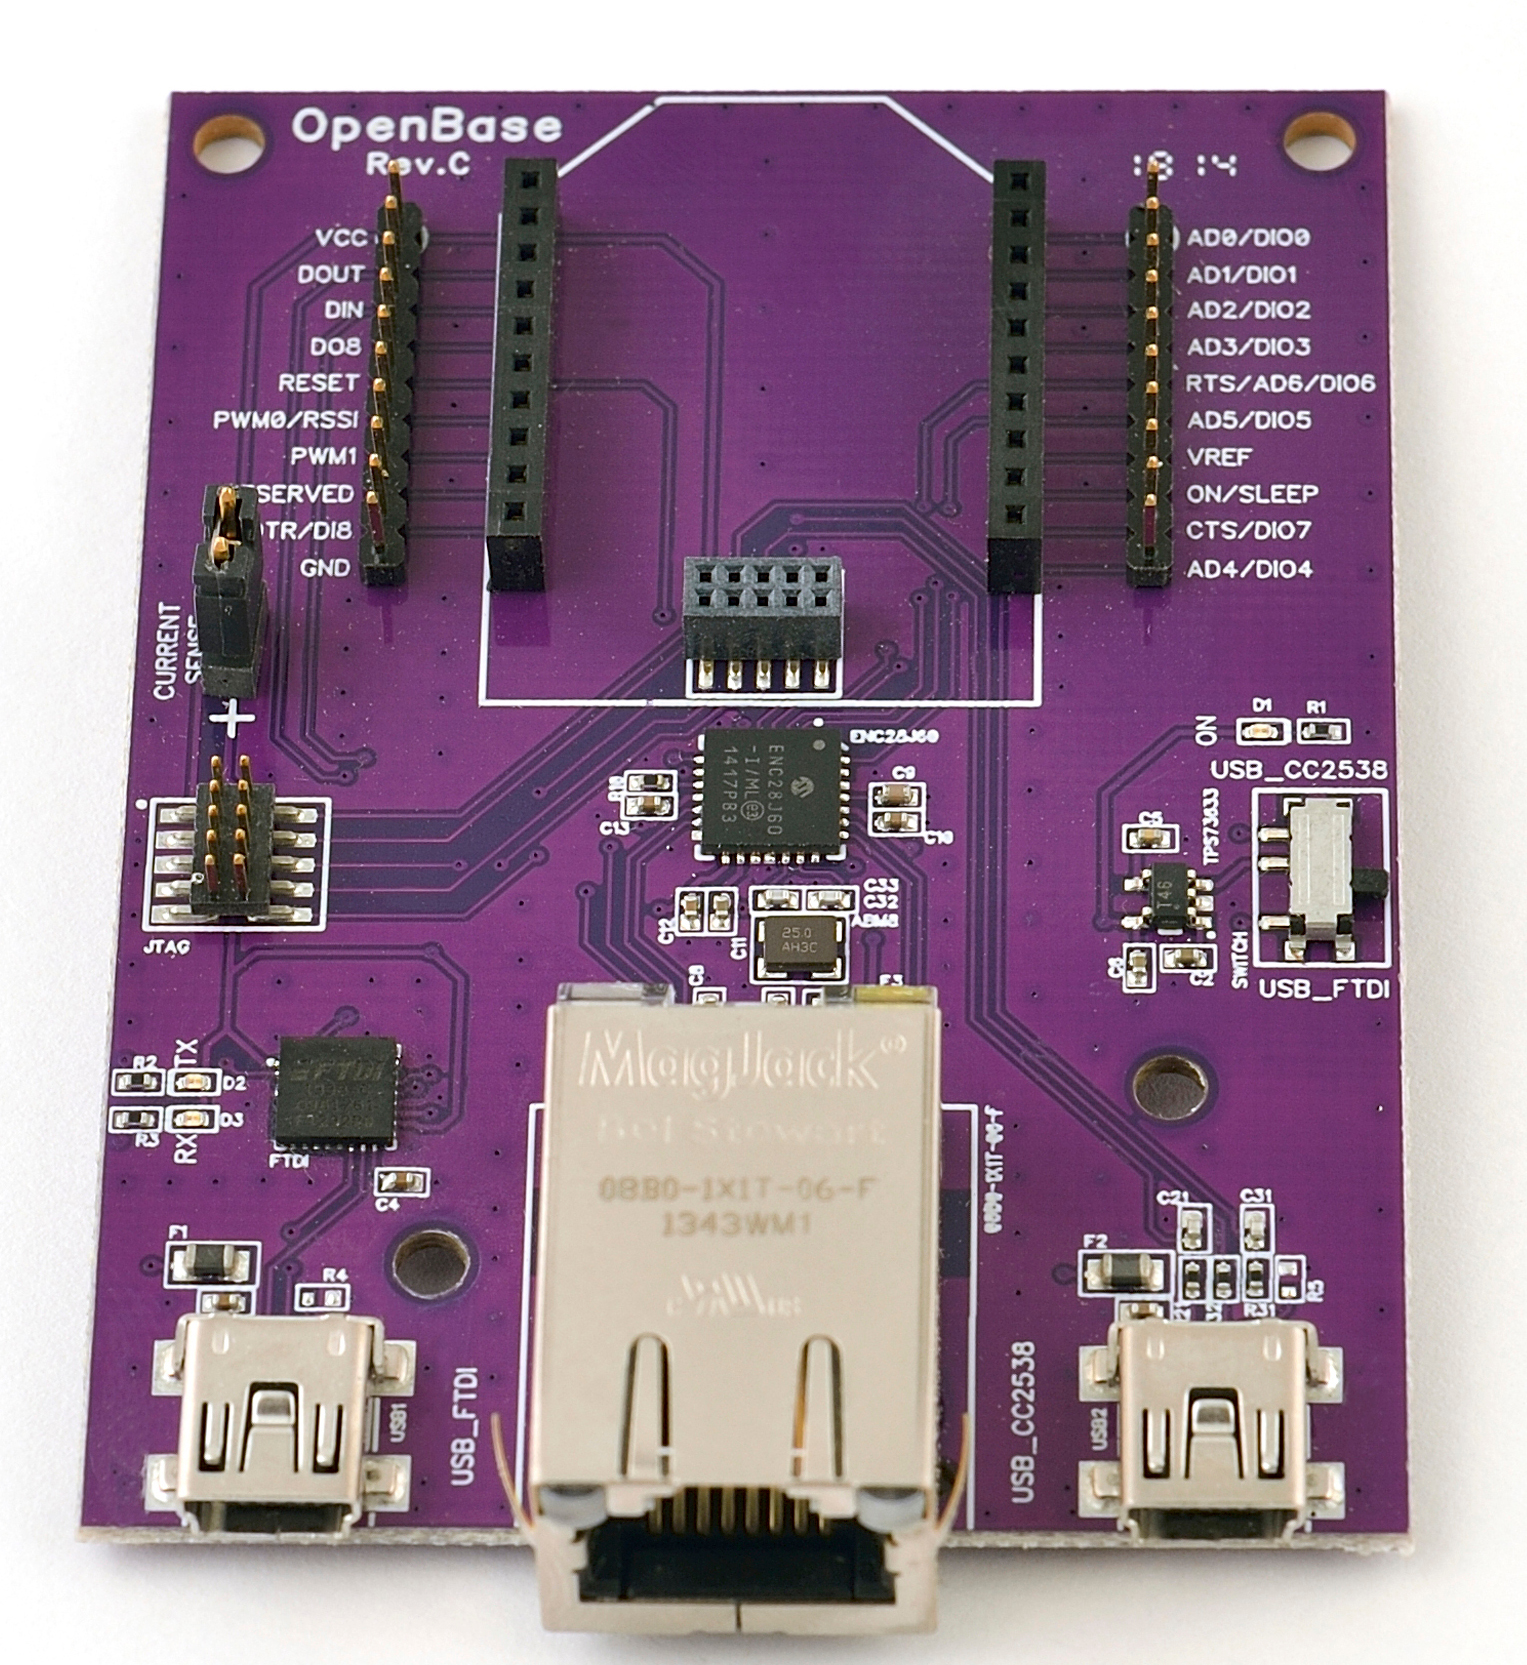
\includegraphics[width=0.35\linewidth]{01-openbase}
    \caption{OpenBase board.}
    \label{fig:openbase}
\end{figure}

%%
% OpenBattery
%%
\section{OpenBattery}
The OpenBattery boards, depicted in Figure~\ref{fig:openbattery}, provides energy to the OpenMote-CC2538 via 2xAAA batteries and provides access to three different sensors via an I2C bus. In particular, the OpenBattery provides a 3-axis acceleration sensor (Analog Devices ADXL346), a light sensor (Maxim MAX44009) and a temperature and relative humidity sensor (Sensirion SHT21). The schematic of the OpenBattery board can be found online in \cite{openbattery_schematic}.

% OpenBattery board
\begin{figure}[!ht]
    \centering
	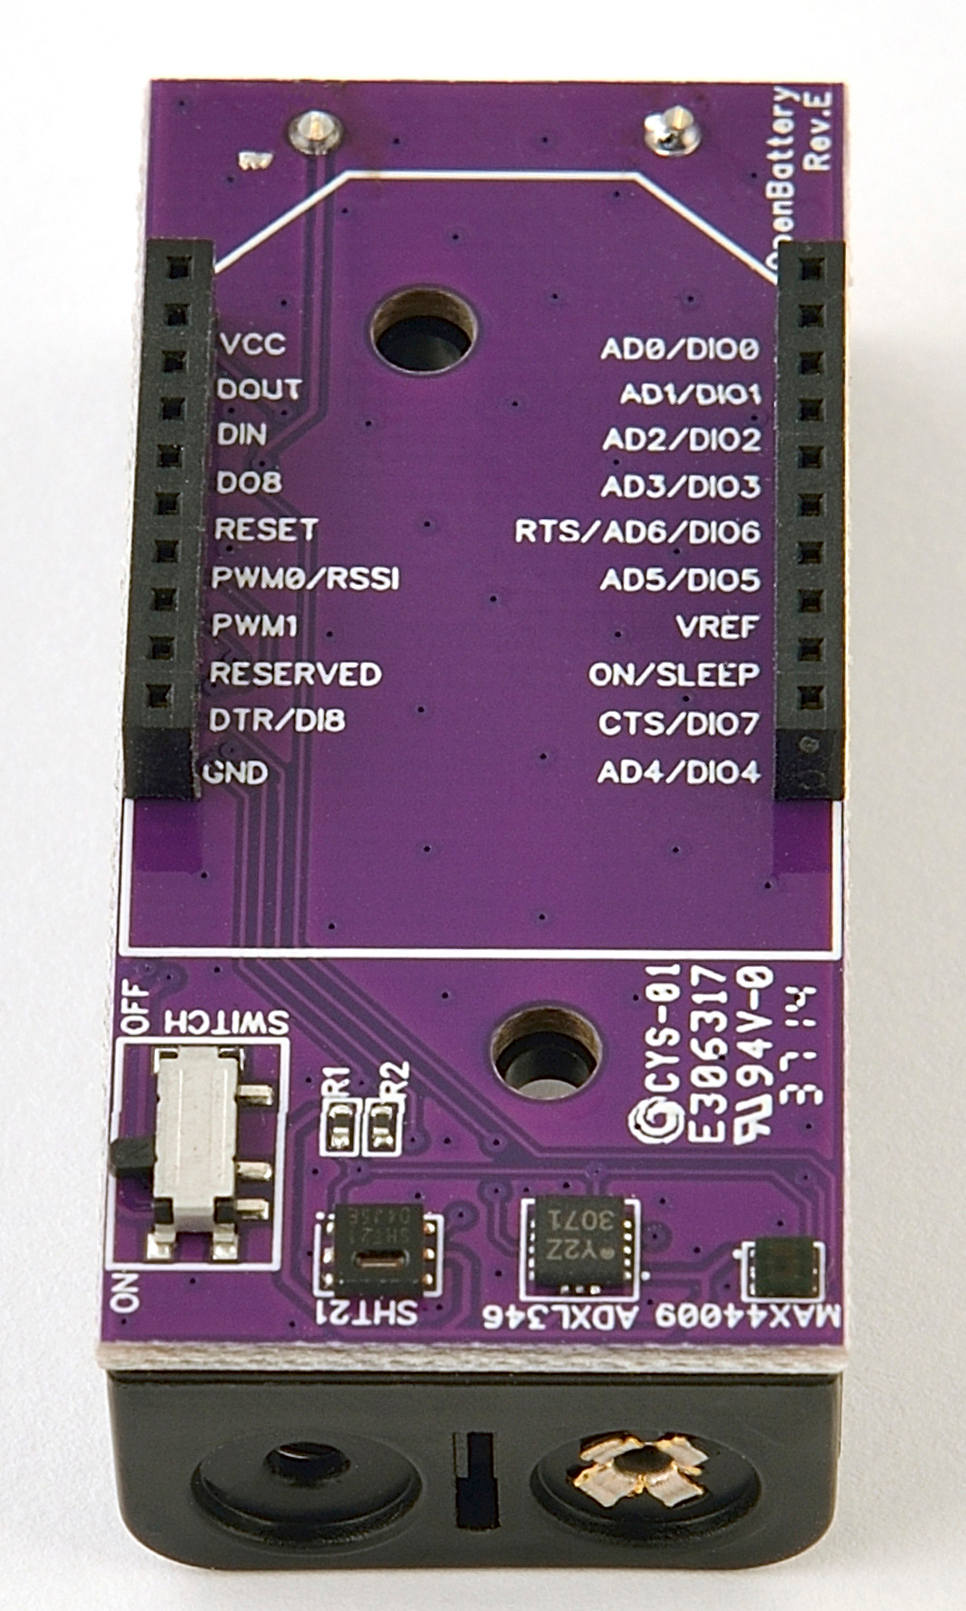
\includegraphics[width=0.25\linewidth]{01-openbattery}
    \caption{OpenBattery board.}
    \label{fig:openbattery}
\end{figure}